\documentclass[handout]{beamer}
\usetheme{Montpellier}
% \usecolortheme{beaver}

\usepackage{beamerthemesplit}
\usepackage{pgfpages}
\usepackage{verbatim}
\usepackage{fancybox}
\usepackage{algorithm}
\usepackage{amsmath}
\usepackage{amsthm}
\usepackage{algpseudocode}
\usepackage{algorithmicx}% http://ctan.org/pkg/algorithmicx
\usepackage{lipsum}% http://ctan.org/pkg/lipsum
\usepackage{xifthen}% http://ctan.org/pkg/xifthen
\usepackage{needspace}% http://ctan.org/pkg/needspace
\usepackage{hyperref}% http://ctan.org/pkg/hyperref
\usepackage{tikz}
\usepackage{mathptmx}
\usepackage[scaled=.90]{helvet}
\usepackage[T1]{fontenc}
\usepackage{framed}
\usepackage{listings}
\usepackage{mdframed}
%-----cut here with a sharp machete or an 19.95 ginsu knife
%************************************************************************
%* BNF.tex								*
%* 									*
%* plain tex macros for formatting grammars				*
%*									*
%* Erik Quanstrom 							*
%* 10. November 1990							*
%************************************************************************

%things to fix:
%	make configurable
%	work with texinfo

\gdef\actifygrammarchars{%
	\catcode`\>\active%
	\catcode`\<\active%
	\catcode`\:\active%
	\catcode`\"\active%
	\catcode`\;\active%
	\catcode`\.\active%
	\catcode`\|\active%
	\catcode`\,\active}

\gdef\deactifygrammarchars{%
	\catcode`\>12%
	\catcode`\<12%
	\catcode`\:12%
	\catcode`\;12%
	\catcode`\.12%
	\catcode`\|12%
	\catcode`\,12}

\newif\ifquote
\quotefalse

\begingroup
   \actifygrammarchars
   \gdef>{\/\endgroup$\rangle$\relax}
   \gdef<{$\langle$\begingroup\sl}
   \gdef:{$\rightarrow$}

   \begingroup
	\catcode`\"\active
	\gdef"{\ifquote%
		'\endgroup\quotefalse%
	   \else%
		\quotetrue\begingroup\deactifygrammarchars\bf`%
	\fi}%
   \endgroup

   \gdef;{\hfill\break}
   \gdef.{\relax}
   \gdef|{$\vert$}
   \gdef,{;\hbox to 1cm{\hfill}}
\endgroup

\def\begingrammar{%
	\begingroup
	\advance\leftskip by 1cm%
	\parindent=-1cm%
	\actifygrammarchars%
	\def\endgrammar{\endgroup}
	\parskip 1ex%
	\relax
}

%
%
%
\def\ul{\lower .2ex\hbox to 1ex{\hrulefill}\relax}%




\title[NDN Gateway]{Multipurpose IP/NDN Gateway and Bridge \\ for Heterogeneous Network Interoperability}
\institute[Donald Bren School of Information and Computer Sciences \\ UC Irvine]{}
\date{\today}
%\subtitle{}
\author[Christopher A. Wood]{Christopher A. Wood \\ \url{www.christopher-wood.com} \\ {\tt woodc1@uci.edu}}
%\institute[]{}
\date{\today}

\begin{document}

%%%%%
%%
%% Resource link: http://www.math-linux.com/spip.php?article77
%%
%%%%

\begin{frame}
	\titlepage
\end{frame}

% \begin{frame}{Agenda}
% 	\tableofcontents
% \end{frame}

%% 6-8 slides each

\section{Overview}
\begin{frame}{Today's Internet: Communication Networks as Distribution Networks}
	The communication-centric design enables point-to-point communcation between any two parties:
	\begin{itemize}
		\item Names and interfaces
		\item Supports end-to-end conversations
		\item Provides unreliable packet delivery via IP datagrams
		\item Compensates for simplicity of IP via complexity of TCP
	\end{itemize}

	Important observation: Helped facilitate today's concent-centric world, \emph{but was never designed for it!}

	\medskip

	\emph{NDN is a new architecture designed for content-centric networking}
\end{frame}

% \begin{frame}{Data vs Communication Networks}
% 	Distribution/data (DN) and communication (CN) networks differ in several key ways:
% 	\begin{table}
% 		\begin{tabular}{c|c|c} \hline
% 		~ & CN & DN \\ \hline
% 		Naming & Endpoints & Content \\
% 		Memory & Invisible \& limited & Explicit (storage = wires) \\
% 		Security & Communication process/channel & Content \\ \hline
% 		\end{tabular}
% 	\end{table}
% \end{frame}

\begin{frame}{NDN Overview}
	Content-centric networking flips around the host-based model of the Internet architecture
	\begin{itemize}
		\item \emph{Content names}, rather than content locations, become addressable. 
		\item Content is retrieved via \emph{interests}, which are similar to URLs: 
		\begin{center}
			{\tt ccnx://rit/gccis/cs/spr/ramsey\_survey}
		\end{center}
		\item The network is permitted to store (cache) content that is in high demand
		\item End result: less traffic to/from the content's original source, better usage of network resources, less latency, etc etc.
	\end{itemize}
\end{frame}

% \begin{frame}{NDN Overview (continued)}
% 	How is data actually retrieved? 
% 	\begin{itemize}
% 		\item A consumer $C$ sends out an \emph{interest} for content they desire.
% 		\item A router $R_i$ use the information in their forwarding information base (FIB) table and data in cached in their content store (CS) to handle incoming interests:
% 		\begin{enumerate}
% 			\item If content with the same name matches what's stored in the CS, return that content
% 			\item Else, store the interest in their pending interest table (PIT) (including the downstream router $R_{i-1}$ or consumer $C$ that made the request), and forward the request upstream to the next router $R_{i+1}$ based on their FIB.
% 			\item FIBs are configured using protocol similar to OSPF
% 		\end{enumerate}
% 		\item Once the interest is satisfied in $R_i$, the PIT entry is cleared, the content is cached, and the data is sent downstream to $C$ or $R_{i-1}$. 
%  	\end{itemize}
% \end{frame}

% \begin{frame}{Interest Format}
% 	\begin{itemize}
% 		\item Interests are similar to URLs: 
% 		\begin{center}
% 			{\tt ccnx://rit/gccis/cs/spr/ramsey\_survey}
% 		\end{center}
% 		\item The {\tt /} character is a delimeter that separates name \emph{components}
% 		\item A component can be \emph{anything}, including binary data (e.g. ciphertext)
% 		\item Interests are matched to providers in FIBs using a standard longest-prefix rule (to my knowledge, interests in CSs must match completely)
% 	\end{itemize}
% \end{frame}

%% TODO: images of this happening 
% \begin{frame}
% 	\frametitle{NDN in Action - \#1}
% 	\begin{figure}[h]
% 		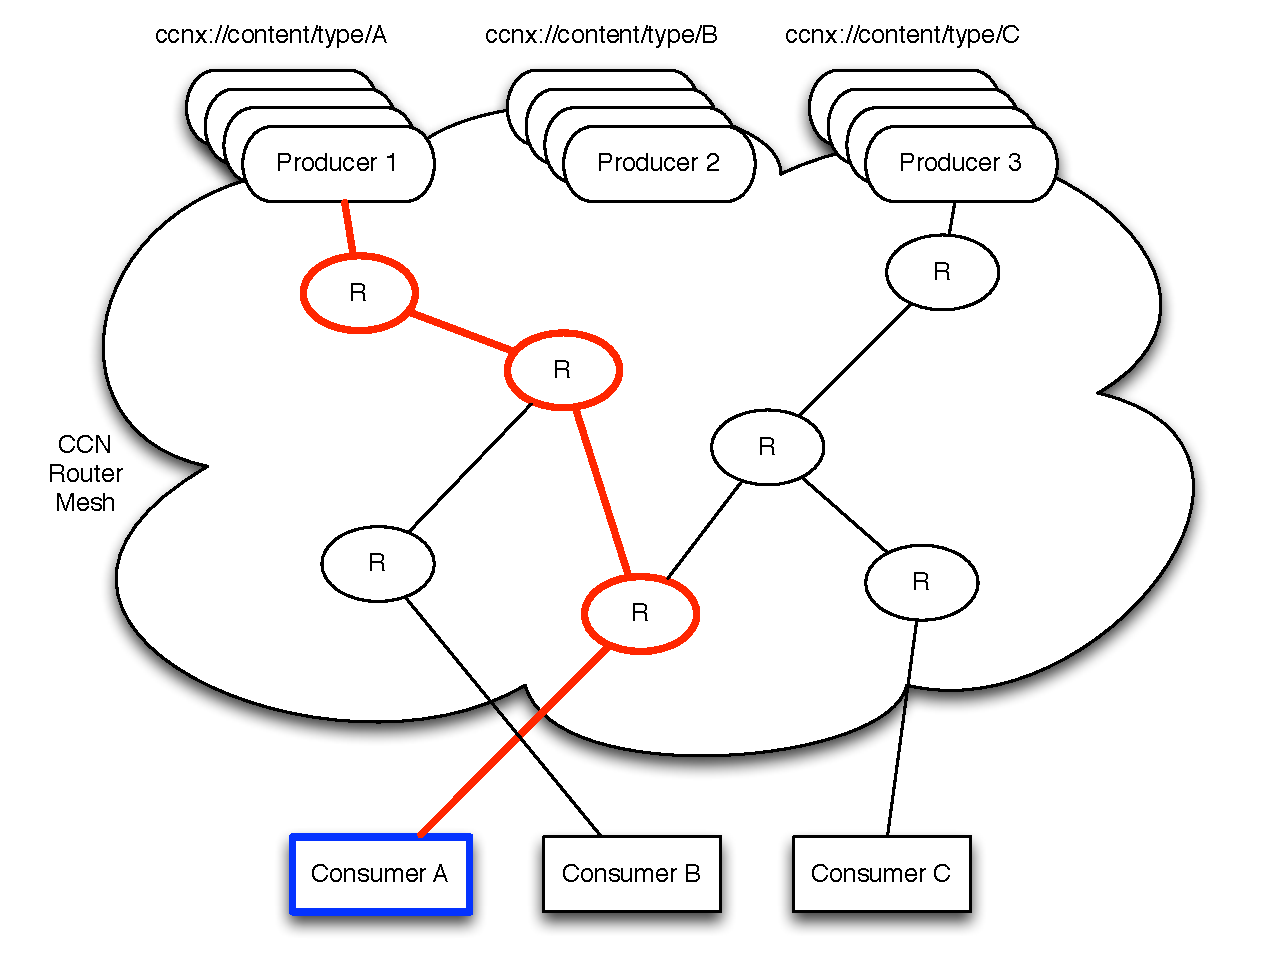
\includegraphics[scale=0.4]{img/ccn_img1.pdf}
% 	\end{figure}
% \end{frame}

% \begin{frame}
% 	\frametitle{NDN in Action - \#2}
% 	\begin{figure}[h]
% 		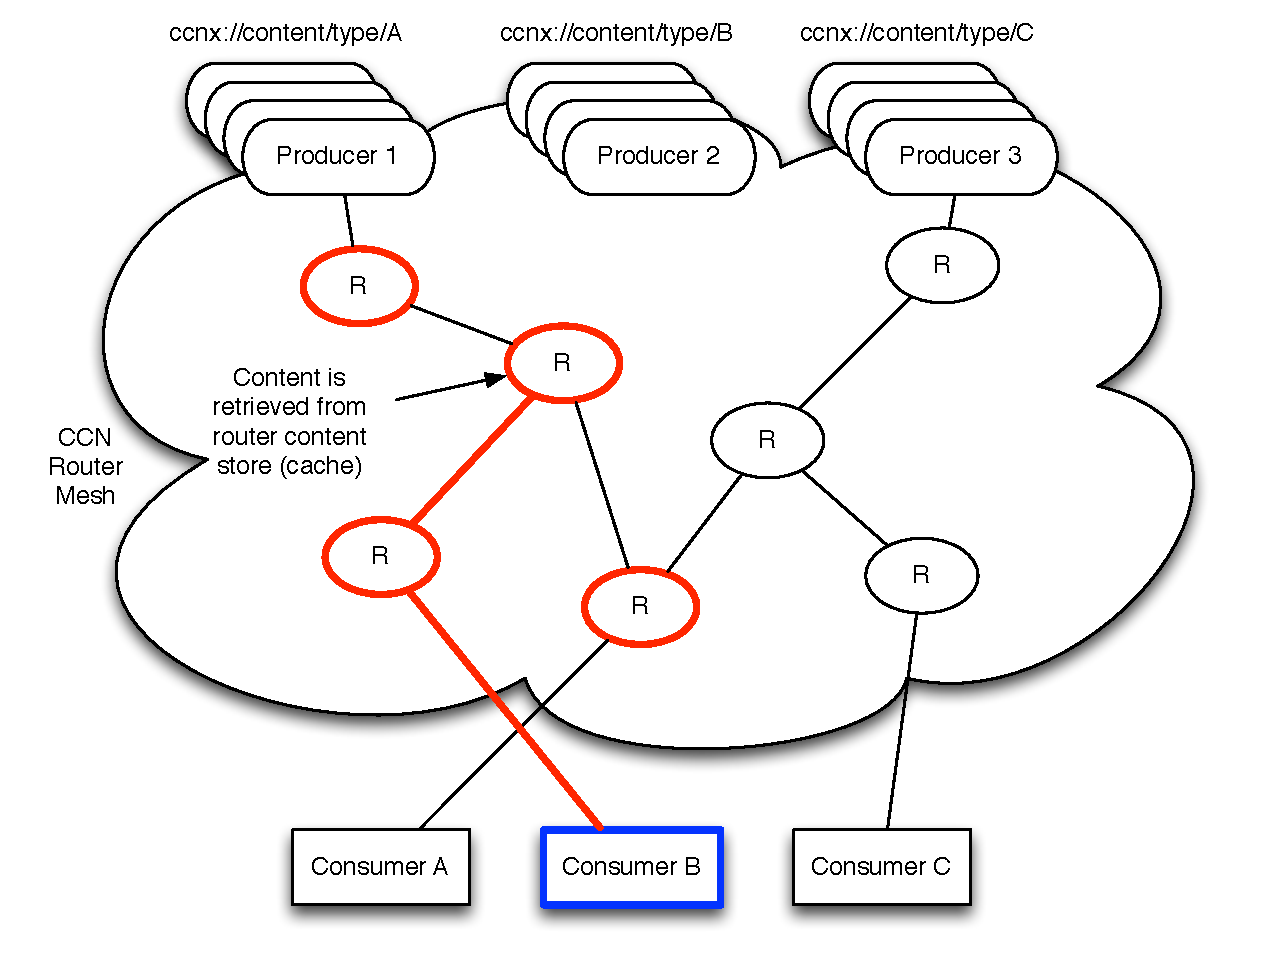
\includegraphics[scale=0.4]{img/ccn_img2.pdf}
% 	\end{figure}
% \end{frame}

% \begin{frame}
% 	\frametitle{NDN in Action - \#3}
% 	\begin{figure}[h]
% 		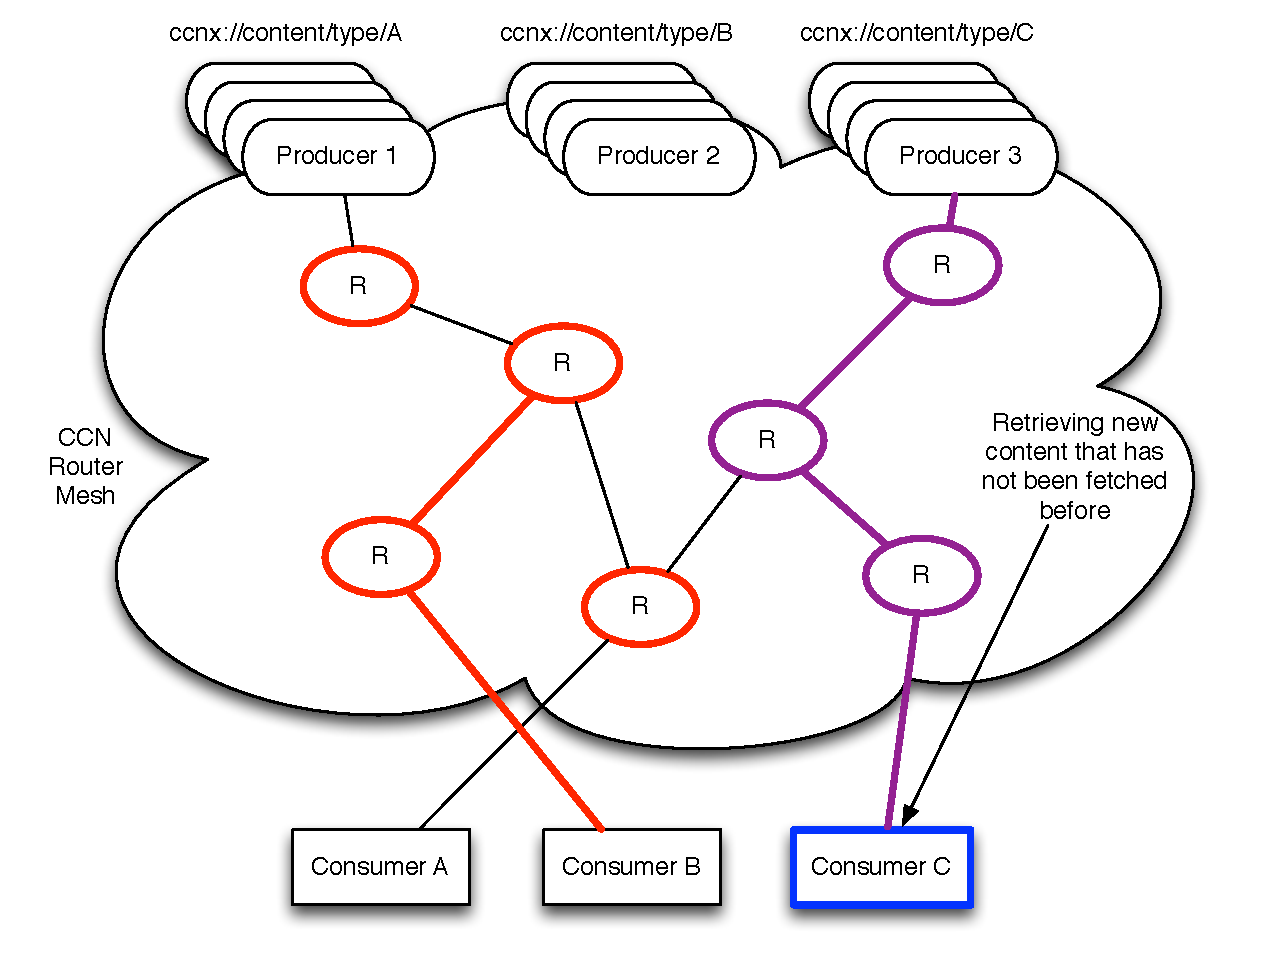
\includegraphics[scale=0.4]{img/ccn_img3.pdf}
% 	\end{figure}
% \end{frame}

% \begin{frame}
% 	\frametitle{NDN in Action - \#4}
% 	\begin{figure}[h]
% 		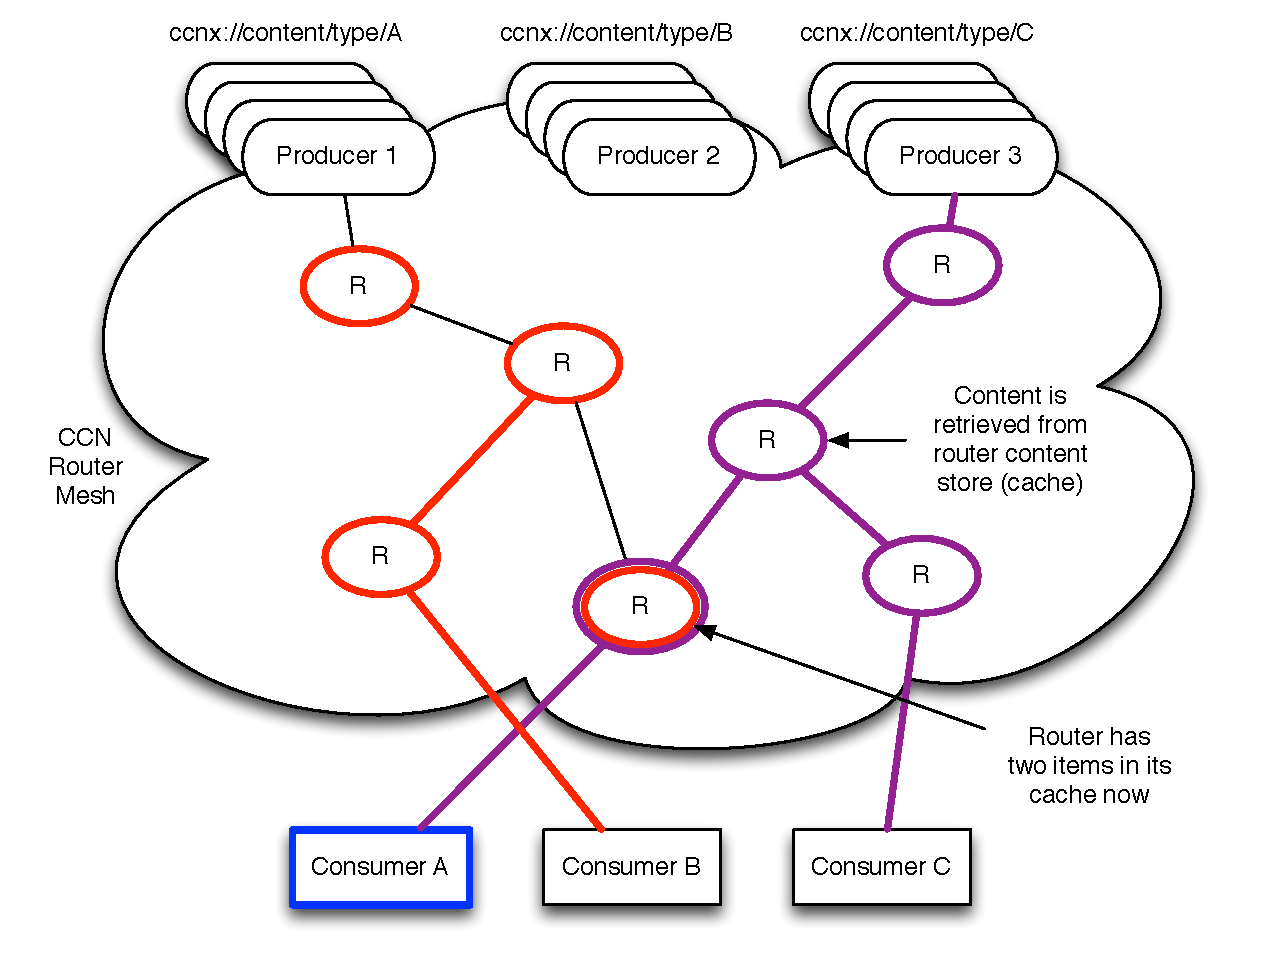
\includegraphics[scale=0.4]{img/ccn_img4.pdf}
% 	\end{figure}
% \end{frame}

% \begin{frame}{NDN at a Larger Scale}
% 	\begin{figure}[h]
% 		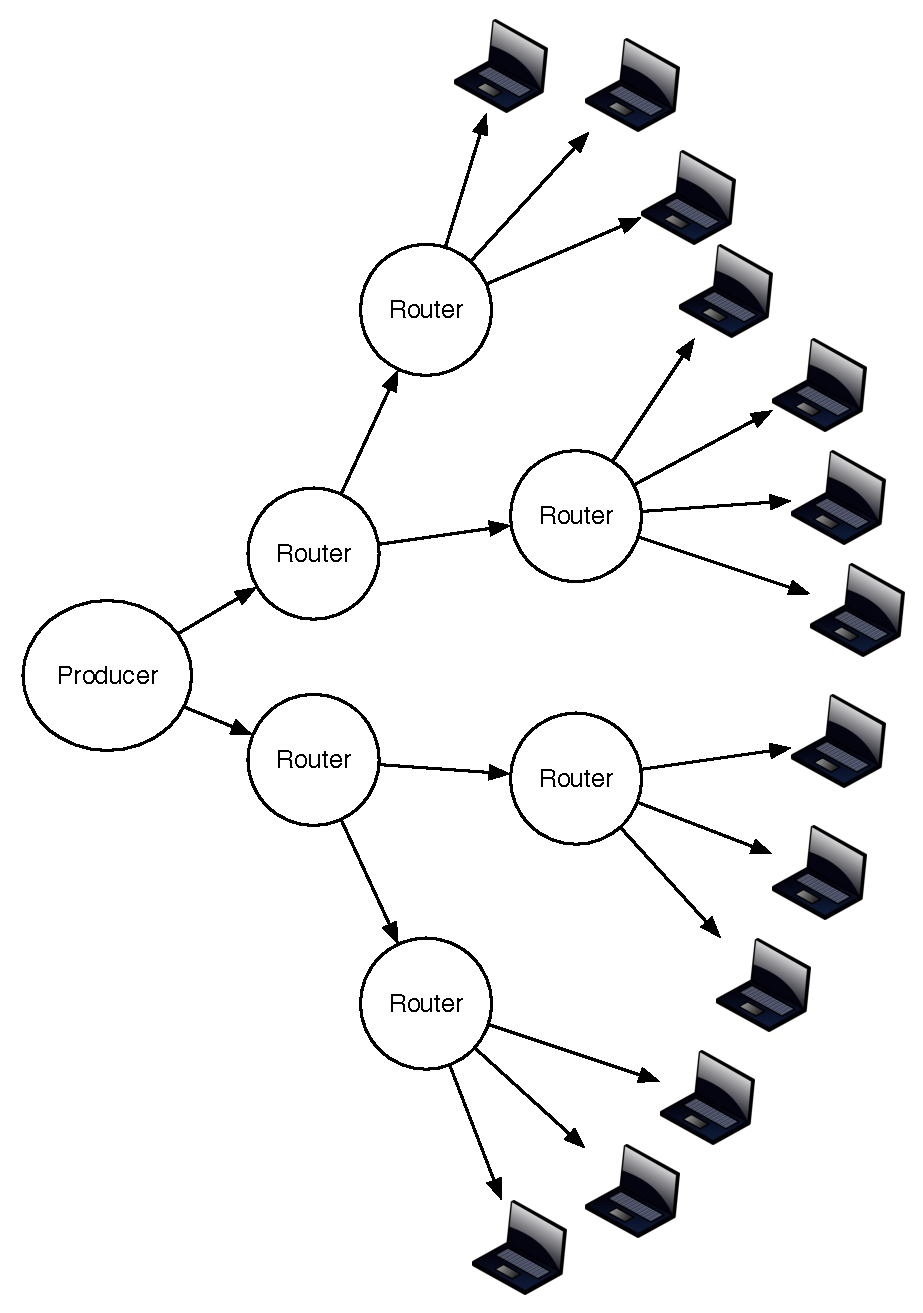
\includegraphics[scale=0.3]{img/ndn_dist.pdf}
% 	\end{figure}
% \end{frame}

\begin{frame}{Motivation for NDN Gateway/Bridge}
	\textbf{Question}: If adopted, how will NDN be deployed?
	\begin{enumerate}	
		\item ``Turn off'' the Internet, swap in new hardware, and then flip the switch again
		\begin{itemize}
			\item Bad idea...
		\end{itemize}
		\item Incrementally ``roll out'' NDN hardware and slowly make it interoperable with existing IP network
		\begin{itemize}
			\item How to enable NDN-based applications to communicate with IP-based applications (and vice versa)?
			\item ...and how to do this without re-writing the transport/network layer of IP-based applications to use CCNx (i.e., implement NDN functionality on top of IP)?
		\end{itemize}
	\end{enumerate}

	{\bf Answer}: Use a NDN-network edge gateways to hide the details of NDN/IP communication mechanics and translate IP messages to compliant NDN interests (and vice versa), and use NDN-network edge bridges to connect isolated NDN ``islands''.
\end{frame}

\section{Modes of Operation}
\subsection{Gateway Functionality}
\begin{frame}{Gateway Semantic Translations}
	\begin{figure}[h]
		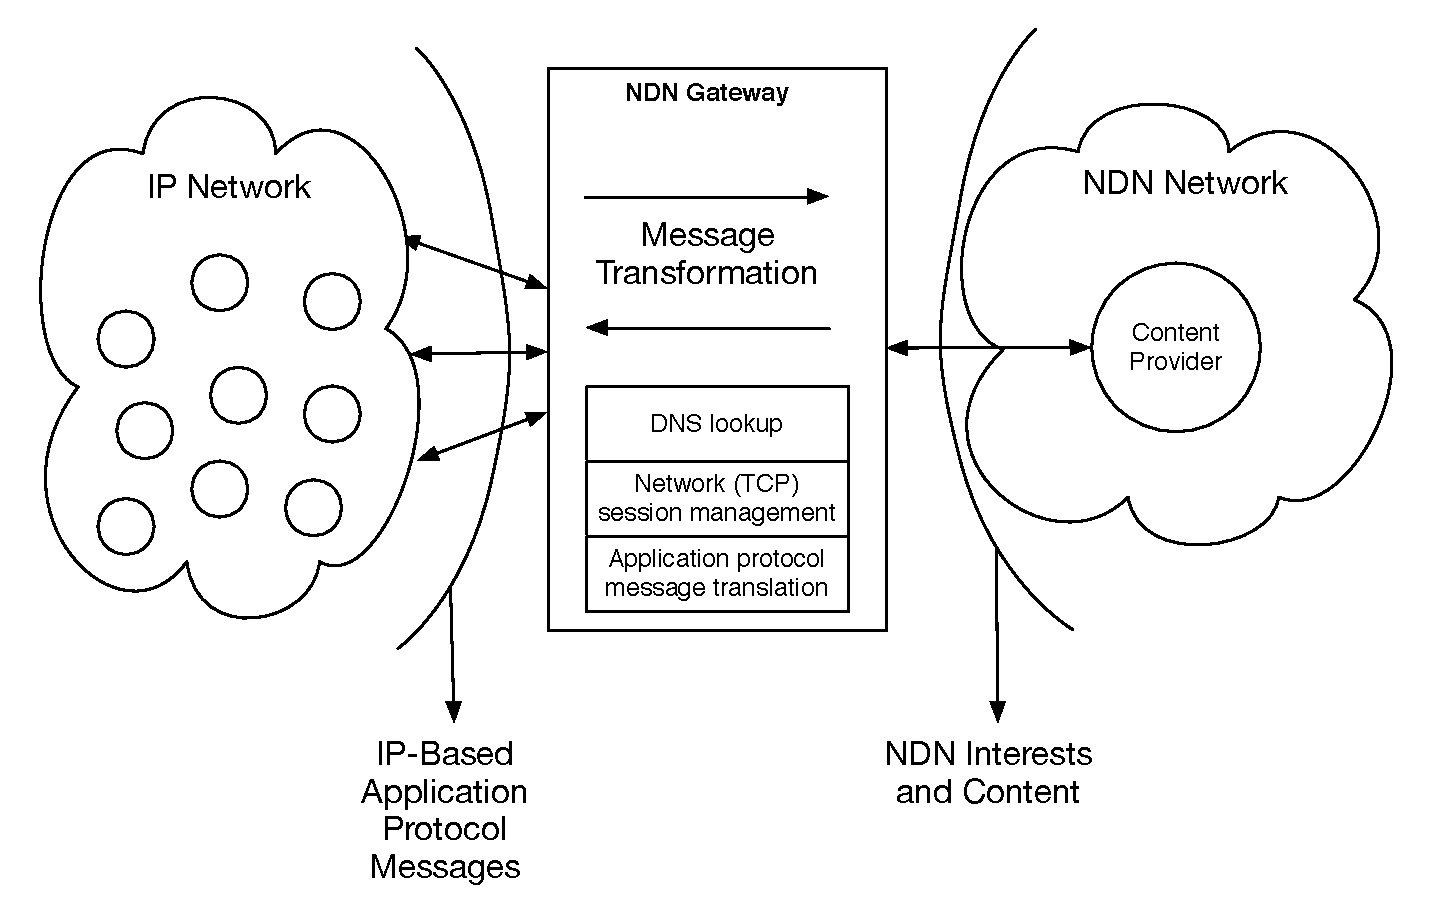
\includegraphics[scale=0.4]{img/gateway_highlevel.pdf}
	\end{figure}
\end{frame}

\begin{frame}{IP-to-NDN Traffic}
	\begin{itemize}
		\item HTTP GET requests issued to get content with a similar name
		\begin{itemize}
			\item e.g., {\tt GET X.X.X.X:80/ndn/ccnx/name/of/content}
			\item The request path is mapped to the outgoing interest name 
		\end{itemize}
		\item TCP connections established to stream data to NDN producers
		\begin{itemize}
			\item Socket connection between IP-based client and gateway established, NDN producer name first sent, and then all remaining data is streamed
			\item The gateway partitions data from the socket and packs it into an interest for the desired NDN producer
		\end{itemize}
	\end{itemize}
\end{frame}

\begin{frame}{NDN-to-IP Traffic}

Interests are encoded according to a special grammar to enable the gateway to parse interests and issue them using the appropriate IP-based protocol

\begin{figure}
\begin{mdframed}
\begingrammar
\noindent
<ip-interest>:	'/$\dots$/ip/'<protocol>.

<protocol>:	'http/'<http-cmd>[{'/'<http-path>}] | 'tcp/'<tcp-ident>'/'<uri-encoded-string>. 

<http-cmd>: 'GET' | 'PUT' | 'POST' | 'DELETE'.

% <ftp-cmd>: 'ascii' | 'binary' | 'bye' | 'cd' | 'close' | 'delete' | 'get' | 'help' | 'lcd' | 'ls' | 'mkdir' | 'mget' | 'open' | 'put' | 'pwd' | 'quit' | 'rmdir'.

<http-path>: <uri> | <ip-address>[port]['/'<uri-encoded-string>]

<tcp-ident>: <SHA256-hash>'/'<nonce>. % nonce is the random ID associated with the TCP socket for constant-time lookup when going from ndn-to-ip, this must be set during the connection establishment phase from ip-to-ndn (if it doesn't exist in the TCP state table, then the NDN-side is creating the connection in one shot)

% <tcp-param>: <uri-encoded-string>.

% <uri-encoded-string>: TODO

% <number>:	<real-number>;
% 		"$\{$" <real-number> "," <real-number> "$\}$";
% 		{$\backslash$}b[01][01]+;
% 		{$\backslash$}o[07][07]+;
% 		\$[0-9A-Fa-f][0-9A-Fa-f]+.

%<real-number>:	[\+--]?[0-9][0-9]+[\.[0-9]+]?[[eE][0-9][0-9]+].

% <operator>:	"*" |	 "/"	|     "$\backslash$"	| "\%";
% 		"==" |	 "!="	|     "$>$" 		| "$<$"  
% 		| "$<$=" | "$>$=";
% 		"\ul ="	| "\ul !=" |  "\ul $<$" | "\ul $>$" 
% 		| "\ul$<$=" | "\ul$>$=";
% 		"\&"	 | "$\vert$"  | "$\uparrow\uparrow$";
% 		"\&\&"	| "$\Vert$"  | "\ul$\uparrow$".
		
\endgrammar
\end{mdframed}
\end{figure}

\end{frame}

\subsection{Bridge Functionality}
\begin{frame}{Bridging NDN Islands}
	\begin{figure}[h]
		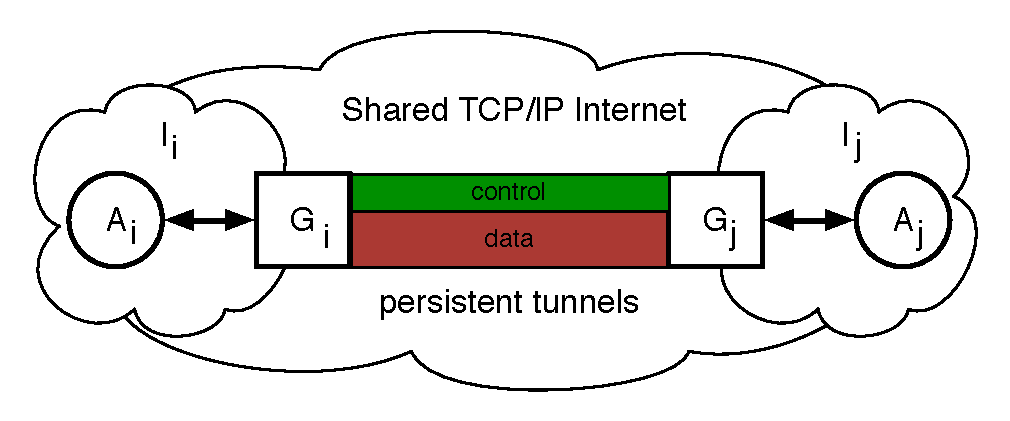
\includegraphics[scale=0.5]{img/island_tunnel.pdf}
	\end{figure}
\end{frame}

% \section{Internal Design}
% \begin{frame}{Pipeline-Based Load Balancing Design}
% 	\begin{figure}[h]
% 		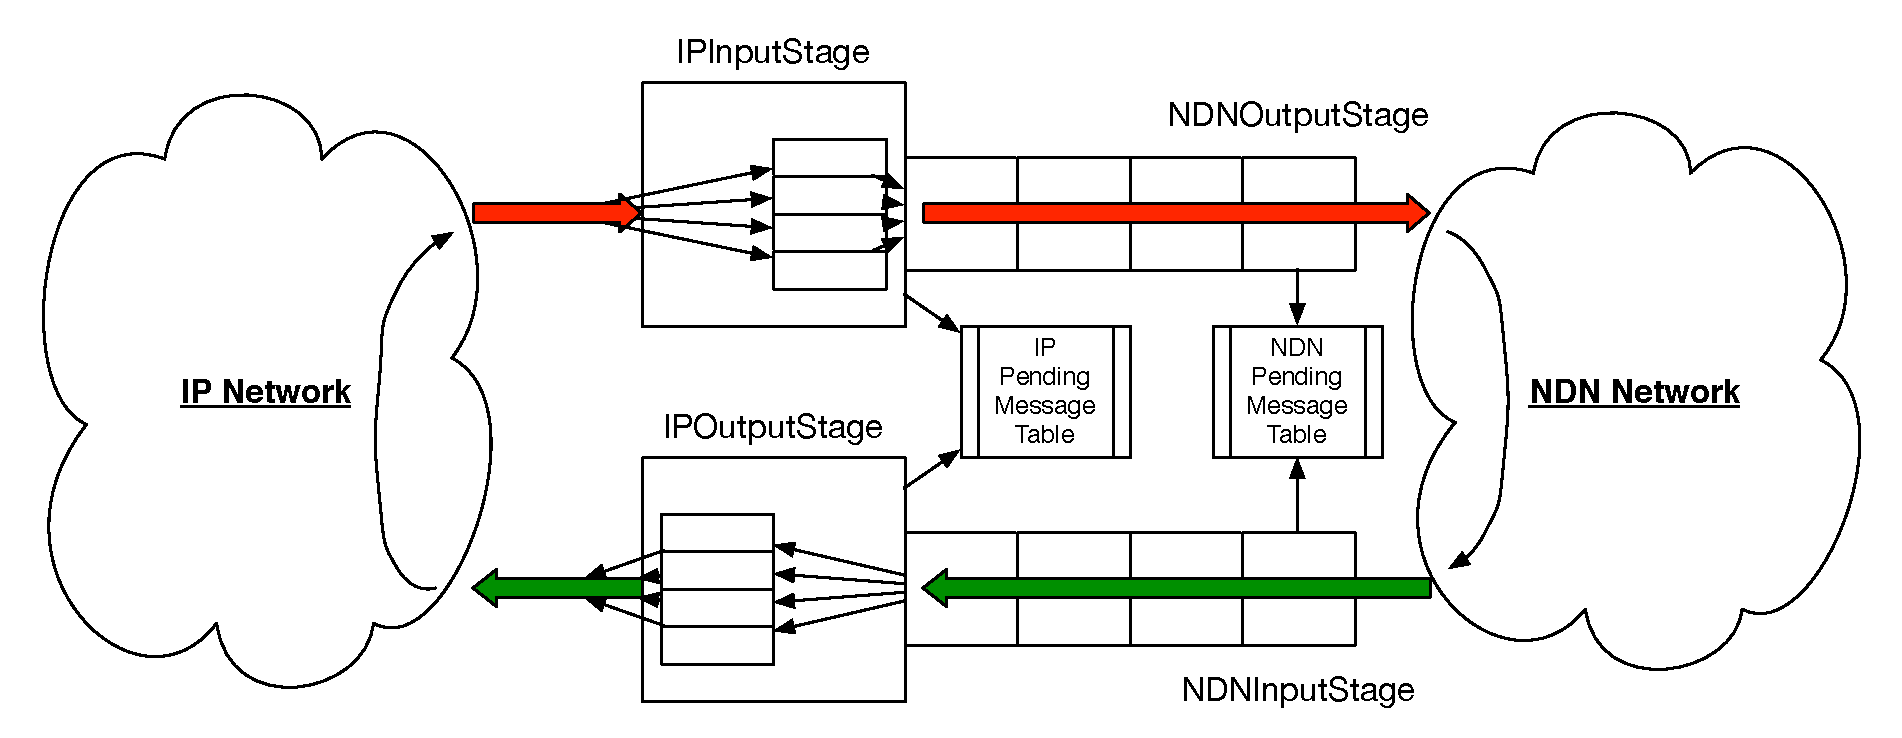
\includegraphics[scale=0.37]{img/pipeline.pdf}
% 	\end{figure}
% \end{frame}

\section{Experimental Setups}
\begin{frame}{Performance Measurement: Experiments and Metrics}
	We will assess the design and implementation performance with the following experiments:
	\begin{itemize}
		\item Bidirectional ``application-layer'' and ``transport-layer'' communication across the gateway
		\item Unidirectional messages sent from IP and NDN hosts
	\end{itemize}
	We will collect the following metrics and model them as a function of the number of gateways $n$ and estimated clients $m$:
	\begin{itemize}
		\item Unidirectional message translation overhead
		\item Unidirectional message trip time
		\item Bridge mode message latency (RTT)
		\item Bridge mode symmetric key establishment overhead time
	\end{itemize}
\end{frame}

%% EXAMPLE REFERENCES 
% \begin{frame}
% 	\frametitle{References}
% 	All images taken from Google Developers documentation: 
% 	\begin{center}
% 		\url{https://developers.google.com/appengine/features/}
% 	\end{center}
% 	% \begin{thebibliography}
% 	% \bibitem CHANGE ME PLEASE
% 	% \end{thebibliography}
% \end{frame}

%% EXAMPLE FIGURE
% \begin{comment}
% \begin{figure}
% \centering
% \includegraphics[scale = 0.6]{images/sub_layer.jpg}
% \end{figure}
% \end{comment}

\end{document}
